%http://neutrino.fnal.gov/events/summer_lecture_series/slides2016/Zarko-Pavlovic-Sources.pdf
%http://microboone-docdb.fnal.gov:8080/cgi-bin/RetrieveFile?docid=5787&filename=bnb-flux-microboone.pdf&version=4
The purpose of this chapter is to describe how the neutrinos studied in subsequently described analyses are produced in the Booster Neutrino Beam-line (BNB) at the Fermi National Accelerator Laboratory. An understanding of how these neutrinos are produced and their flux through the MicroBooNE detector is important to properly interpret the results of the low energy excess analysis and kaon production analysis, described in Chapters \ref{sec:LEEsensitivity} and \ref{sec:LEEsensitivity}. In describing the neutrino production techniques and sources, the reader will be introduced to the systematic uncertainties associated with the neutrino source, both in terms of how they arise, and their magnitude. 

\section{The Booster Neutrino Beam}\label{beam_descript_section}
The Boost Neutrino Beam-line (BNB) collides protons at 8.89 GeV/c momentum from the Fermilab Booster synchrotron with a beryllium target to produce a high flux of neutrinos. The layout of the BNB is shown in Figure \ref{BNB_layout_schematic}, and the relevant steps of the neutrino production process will be described in the following sections.

\begin{figure}[ht!]
\centering
	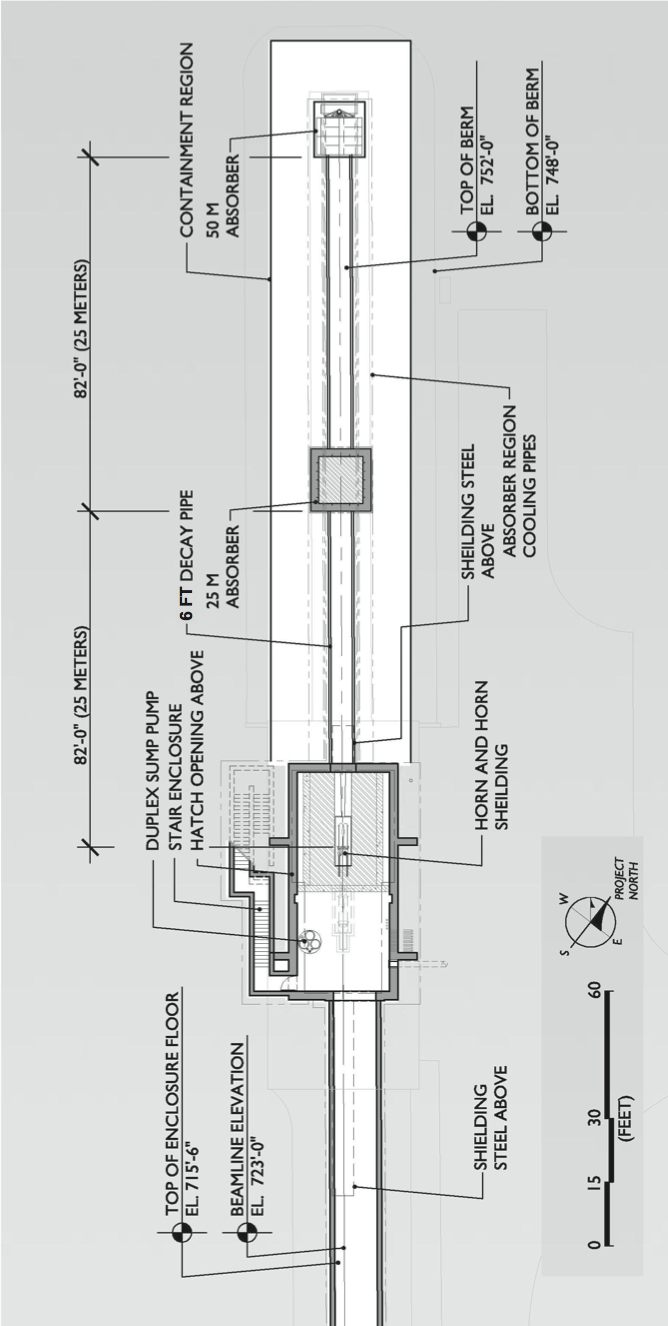
\includegraphics[width=0.5\textwidth]{Figures/BNB_layout_schematic.png} \\
\caption{\textit{Overall layout of the BNB. The primary proton beam, extracted from the Booster, enters the target hall from the left. Upon exiting the target hall, particles encounter a 50-meter-long decay region, terminating in the beam stop on the right. Figure and caption from \protect\cite{MBFluxPaper}.}}\label{BNB_layout_schematic}
\end{figure}

\subsection{Primary Proton Beam}
The protons originate from $H_2$ gas molecules converted to $H^-$ ions via a Cockroft-Walton generator, which are initially accelerated up to approximately 1 MeV kinetic energy. These ions are subjected to a linear accelerator using alternating electromagnetic fields to increase their energy to about 400 MeV. Passing through a carbon foil removes electrons, and the bare protons enter the Booster synchrotron where they are accelerated up to 8.89 GeV/c momentum. The protons are bunched in ``beam spills'' containing roughly $4\times10^{12}$ protons spaced throughout a 1.6 $\mu s$ time window. The protons are then directed towards a thick beryllium target.\\

The absolute number of protons directed on target (POT) is measured by two toroids upstream of the target which part of a larger beam monitoring system. The error on the POT is on the order of 2\%. Additional beam characteristics are monitored by beam position monitors (BPMs), a multi-wire chamber, and a resistive wall monitor (RWM) which together measure beam intensity, timing, width, position, and direction.

\subsection{Proton Target and Focusing Horn}
The beryllium target is 71.1 cm long, which corresponds to 1.7 proton interaction lengths, and is 0.51 cm in radius. Beryllium is chosen as the proton target because it's relatively low Z (4) minimizes radiative losses from the protons before their p-Be interactions which produce secondary mesons ($\pi^\pm$, $K^\pm$, $K^0_L$).\\

The beryllium target is located within a larger focusing electromagnet, referred to as the horn. A schematic drawing of the horn is shown in Figure \ref{BNB_horn_schematic}. The horn is an aluminum alloy pulsed toroidal electromagnet. The pulsed current has a peak at 170 kA and width in time of 143 $\mu s$, coincident with the proton beam arrival time on the target. The current flows along the inner conductor, then returns along the outer conductor. The electromagnetic fields created by this current serve to focus the charged secondaries produced in the p-Be interactions. The direction of this current can be switched to focus the positively charged secondaries, or the negatively charged secondaries, ultimately producing a beam of primarily neutrinos (``neutrino mode'') or of primarily antineutrinos (``antineutrino mode'') respectively.

%\ref{BNB_numode_fig}



\begin{figure}[ht!]
\centering
	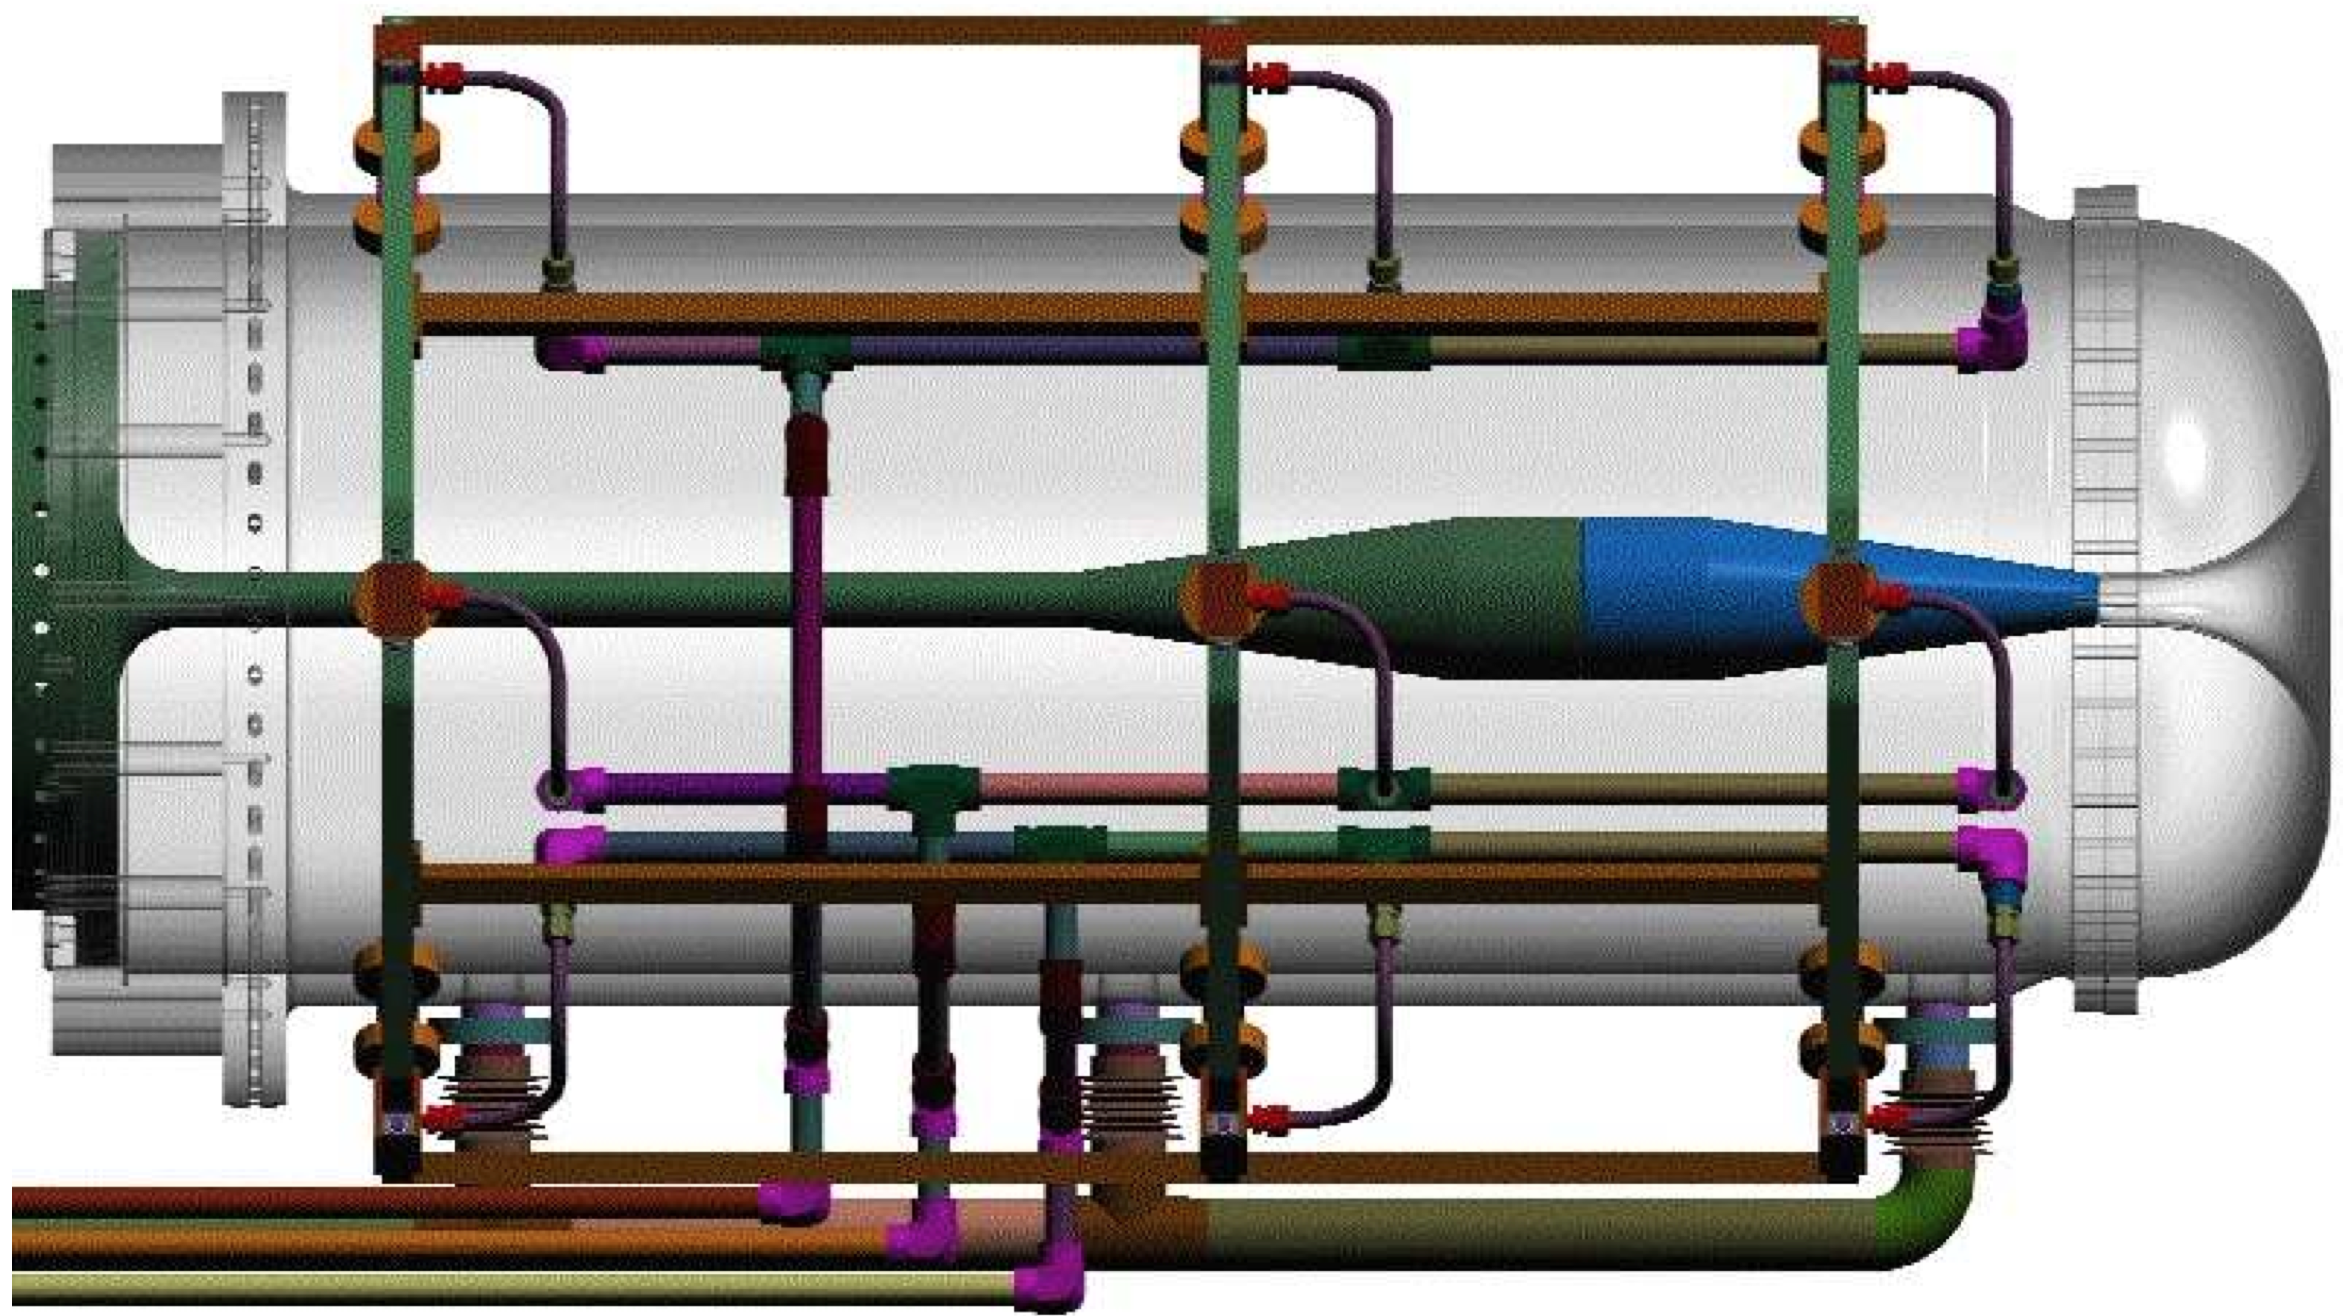
\includegraphics[width=0.7\textwidth]{Figures/BNB_horn_schematic.png} \\
\caption{\textit{The BNB focusing horn system. The gray outer conductor is drawn transparent for visualization purposes. The beryllium target lies within the central hollow tube axis. A current flows along the inner conductor, returning along the outer conductor.}}\label{BNB_horn_schematic}
\end{figure}


\begin{figure}[ht!]
\centering
	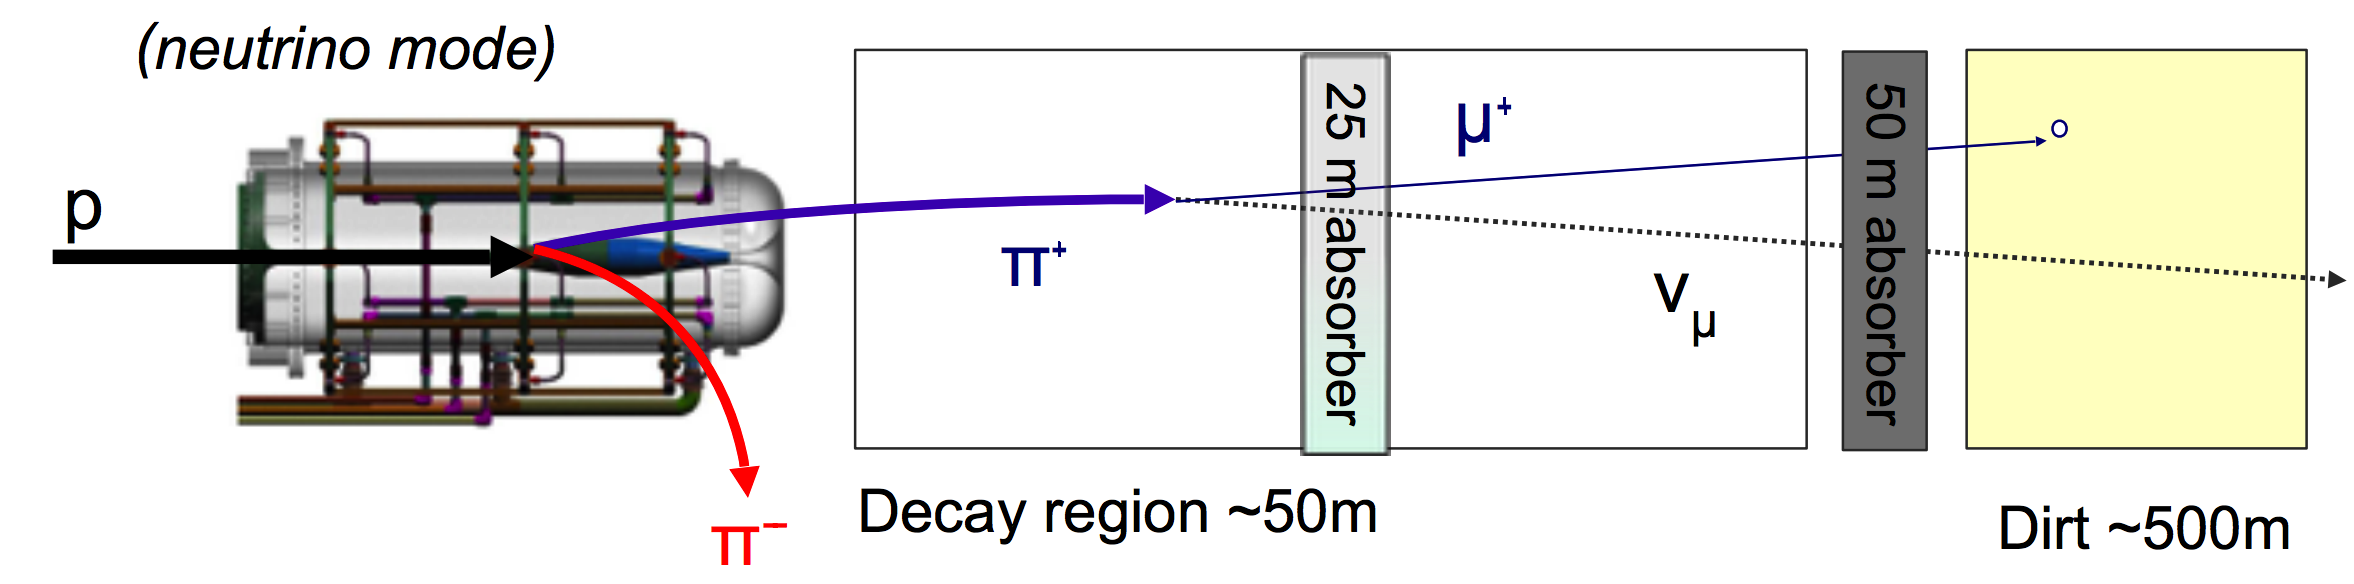
\includegraphics[width=1.0\textwidth]{Figures/BNB_numode_fig.png} \\
\caption{\textit{XXXcaption.}}\label{BNB_numode_fig}
\end{figure}



\section{Neutrino Flux Prediction}\label{beam_flux_descript_section}
